\section{Data Basis}
Here the underlying databasis is analysed. General information is shown in table REF:

\begin{figure}[H] 
 \centering 
 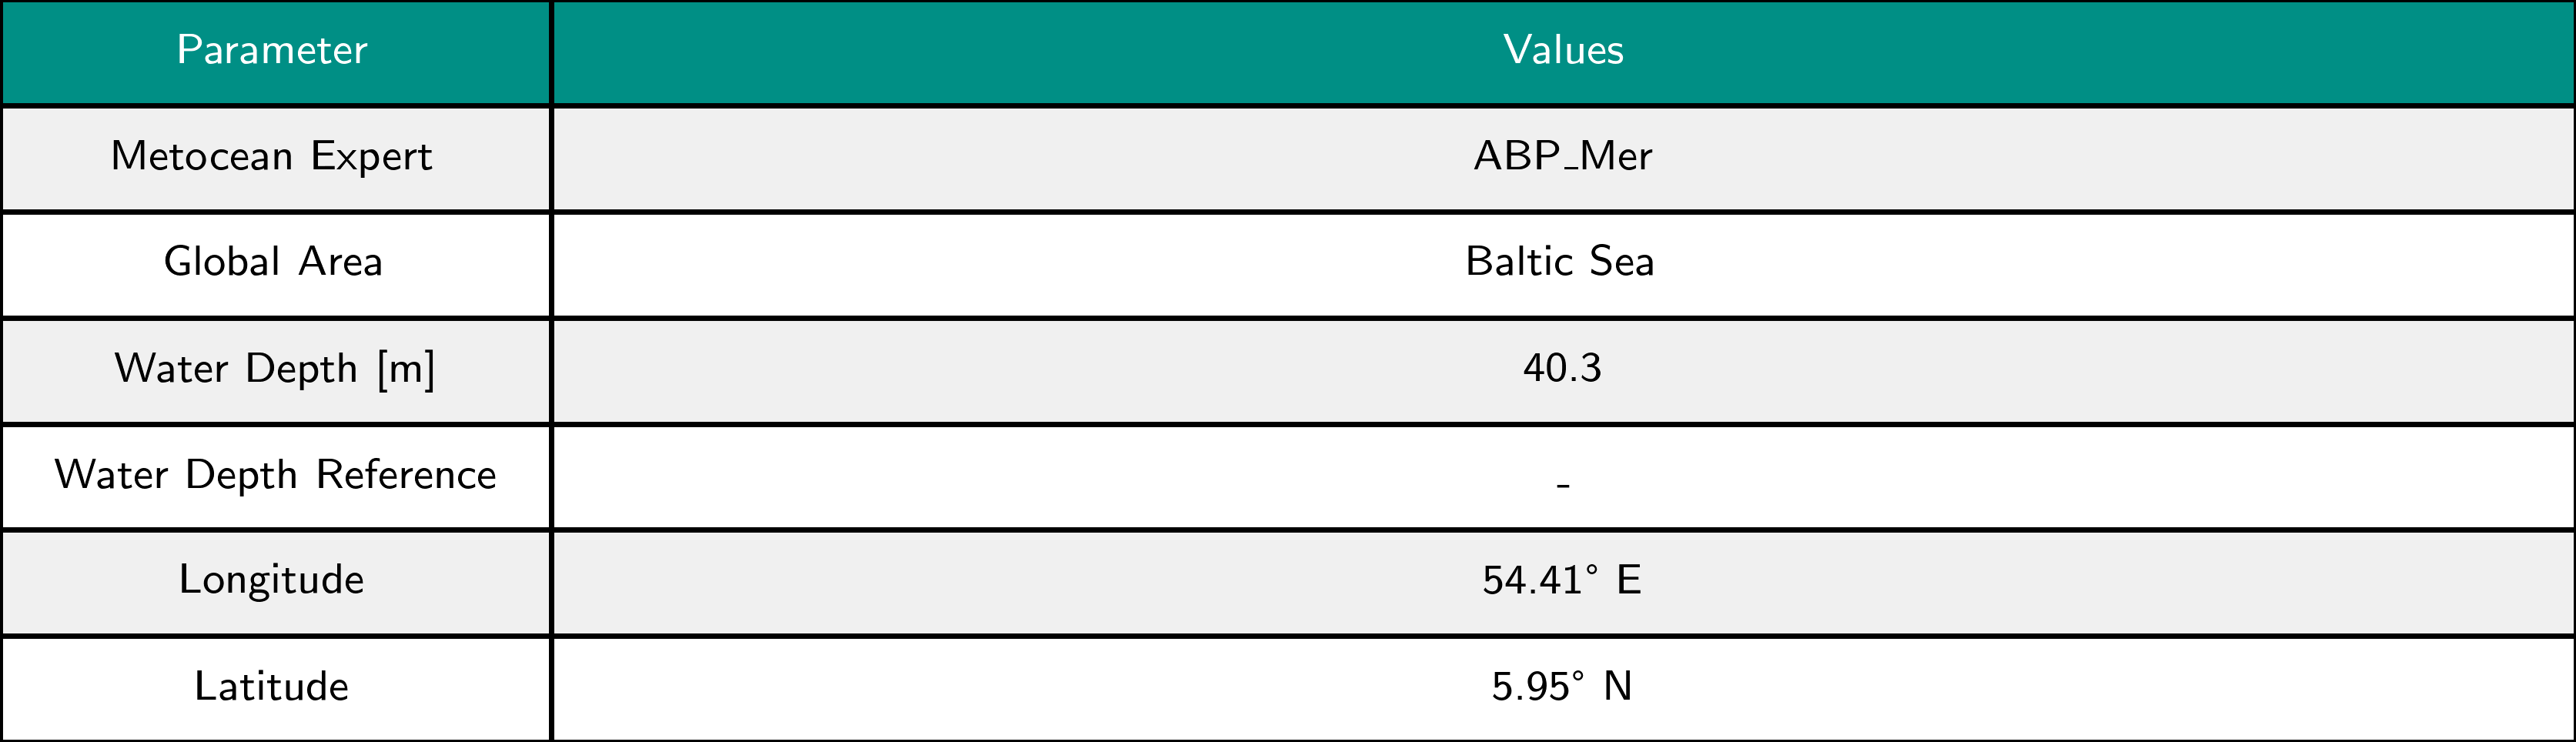
\includegraphics[width=1.0\textwidth ]{C:/Users/aaron.lange/Desktop/Projekte/Hindcast_Tool/HindTool/example_output/DataSorce_global_page_1.png} 
 \captionsetup{type=table} 
\caption{ DataSorce-global-page-1 } 
 \label{tab: DataSorce_global_page_1 } 
\end{figure}

\subsection{Data set overview}

Meta information of the time series data sets considered in this document are specified below in detail. A quality assurance including potential resampling or correction has been conducted. Analysed sensors in the data sets are tabulated in REFERENZ.

\begin{figure}[H] 
 \centering 
 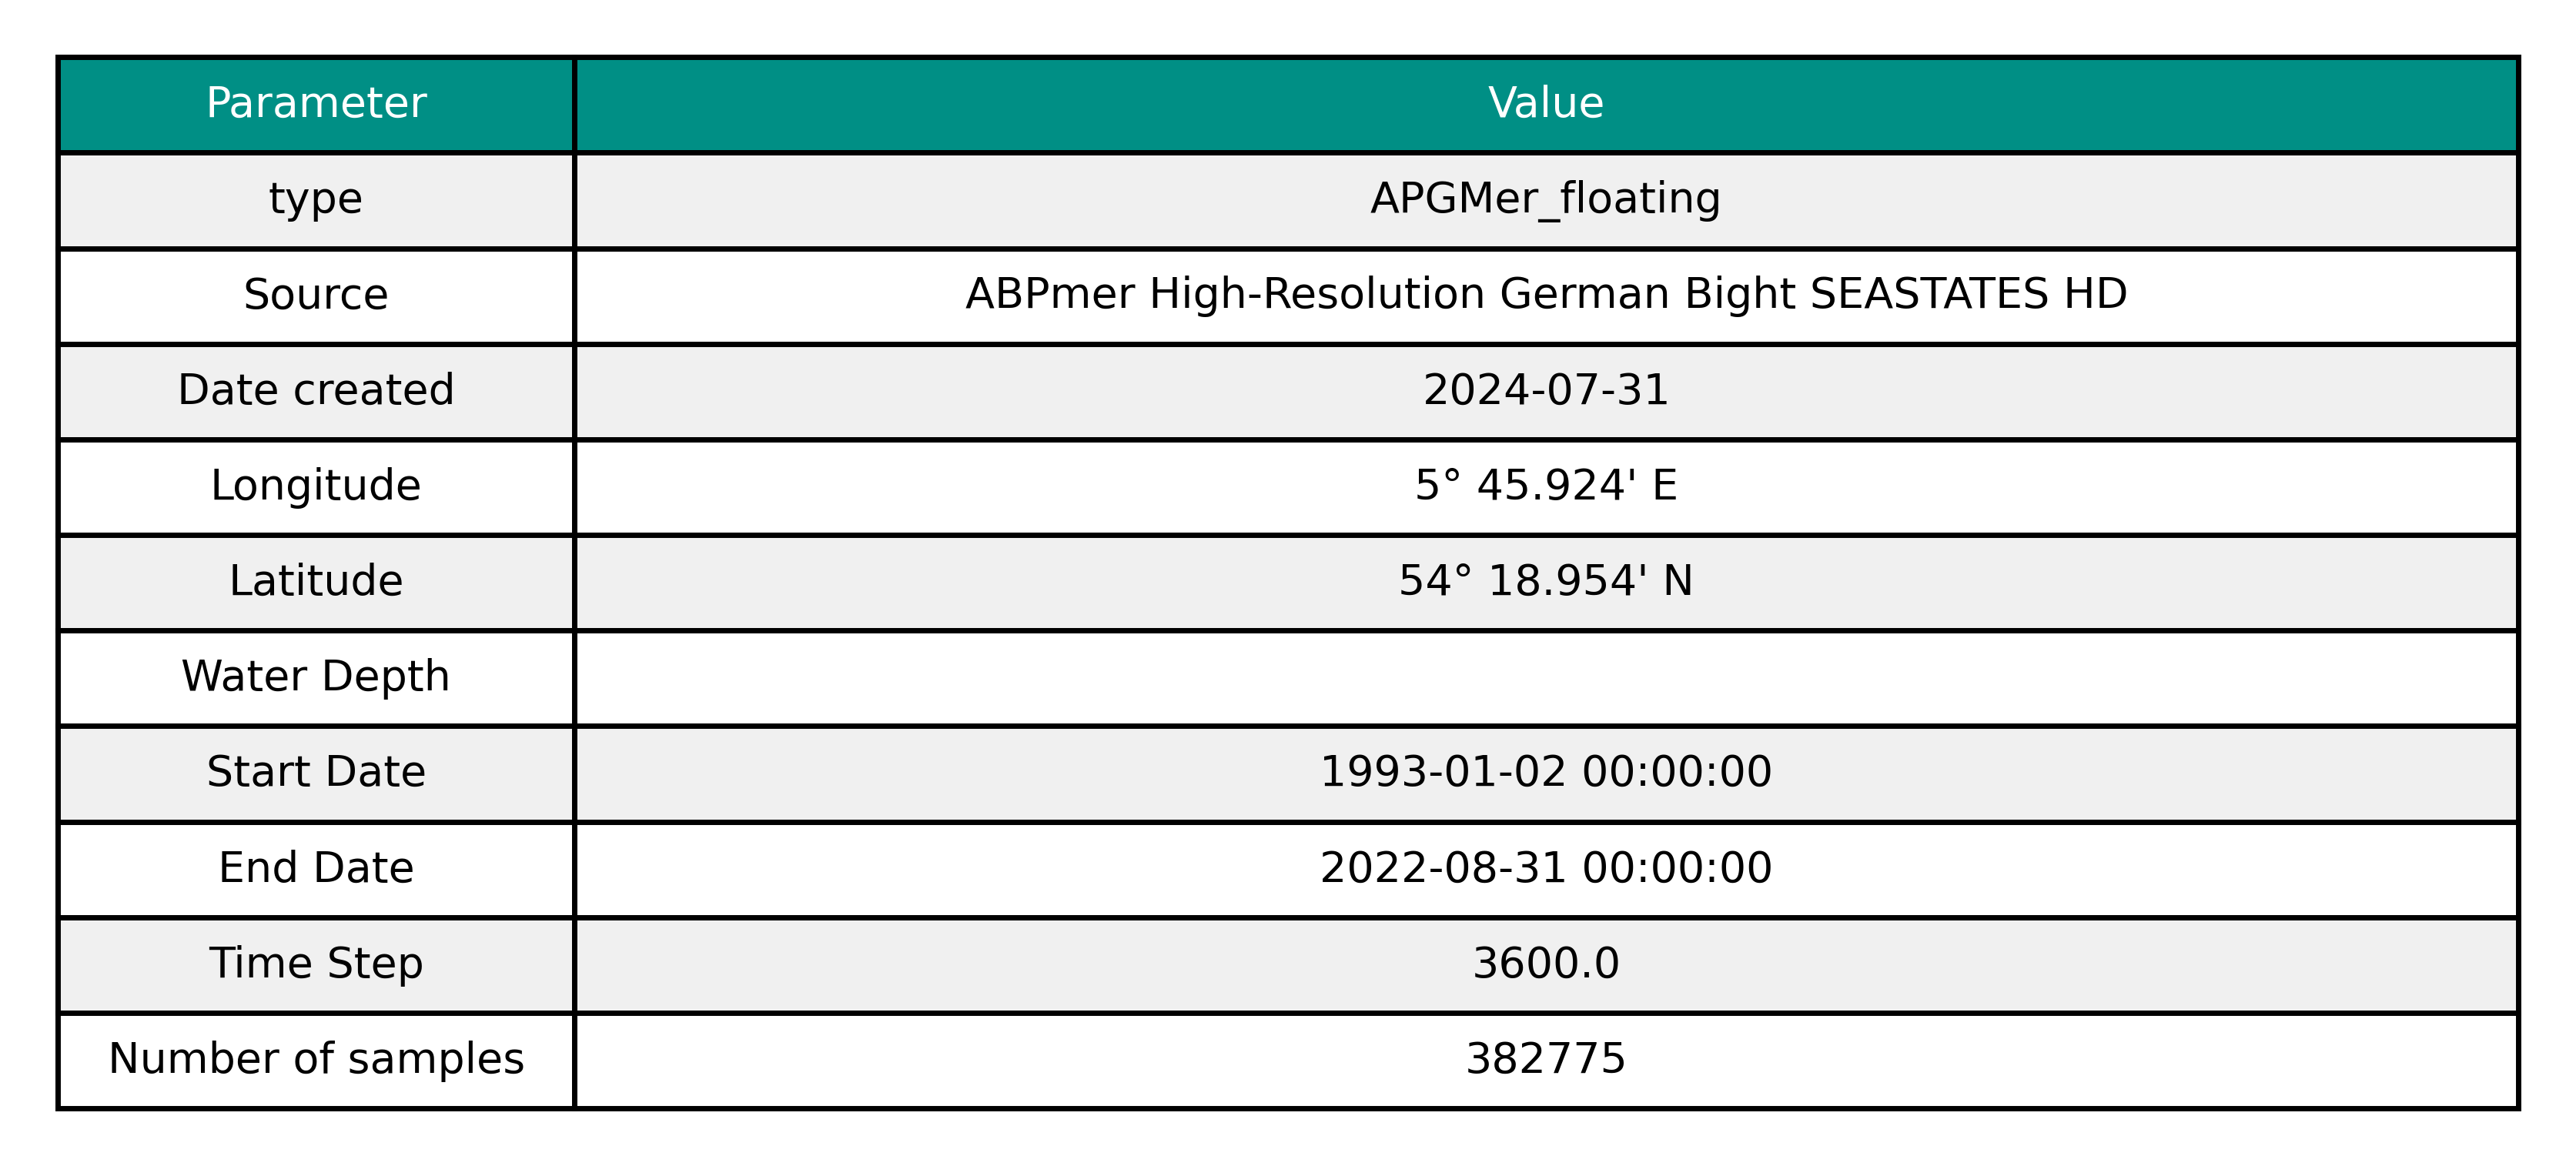
\includegraphics[width=1.0\textwidth ]{C:/Users/aaron.lange/Desktop/Projekte/Hindcast_Tool/HindTool/example_output/DataSorce_Currents_page_1.png} 
 \captionsetup{type=table} 
\caption{ DataSorce-Currents-page-1 } 
 \label{tab: DataSorce_Currents_page_1 } 
\end{figure}
\begin{figure}[H] 
 \centering 
 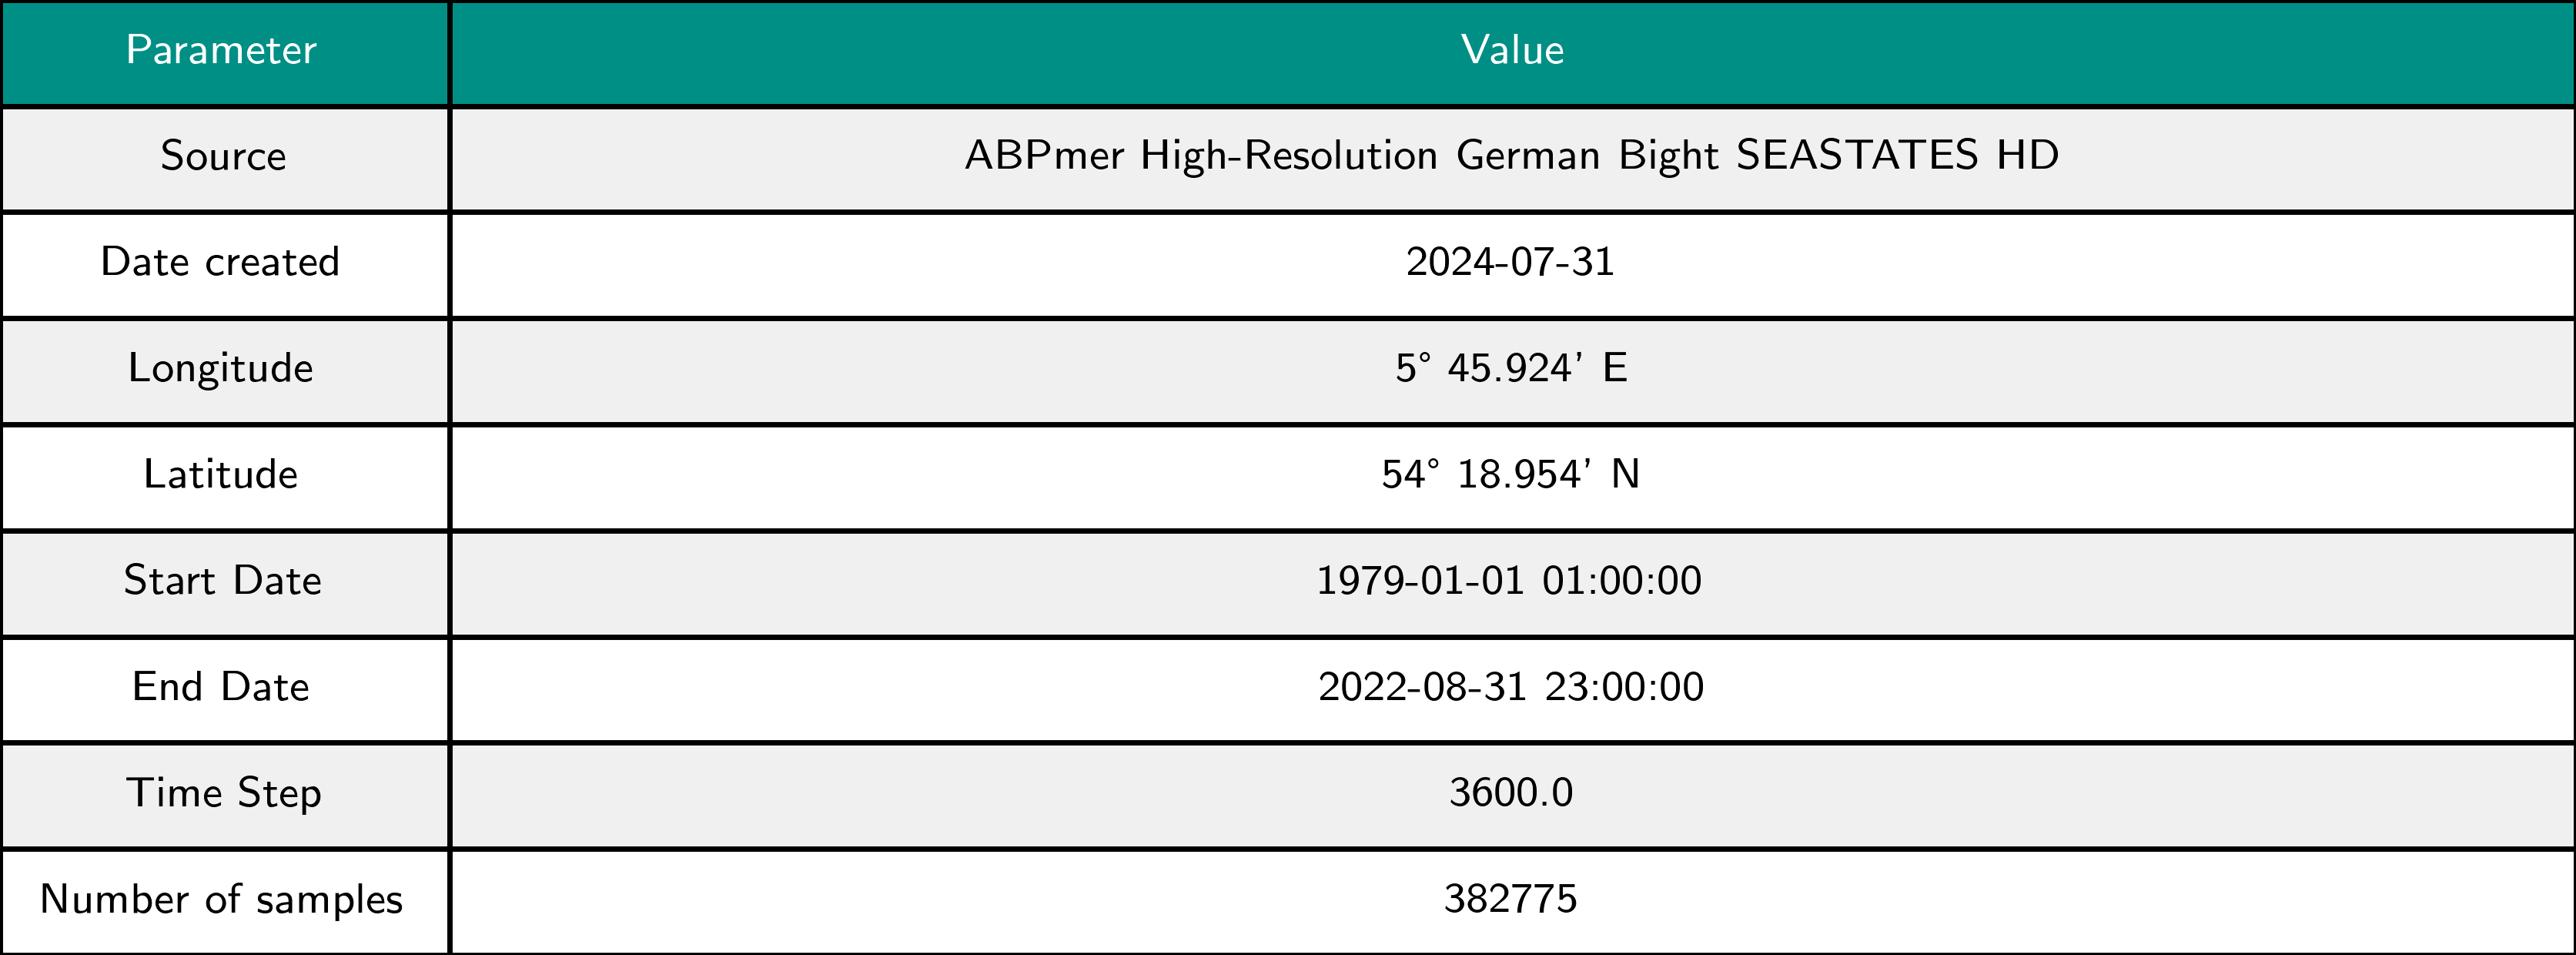
\includegraphics[width=1.0\textwidth ]{C:/Users/aaron.lange/Desktop/Projekte/Hindcast_Tool/HindTool/example_output/DataSorce_Levels_page_1.png} 
 \captionsetup{type=table} 
\caption{ DataSorce-Levels-page-1 } 
 \label{tab: DataSorce_Levels_page_1 } 
\end{figure}
\begin{figure}[H] 
 \centering 
 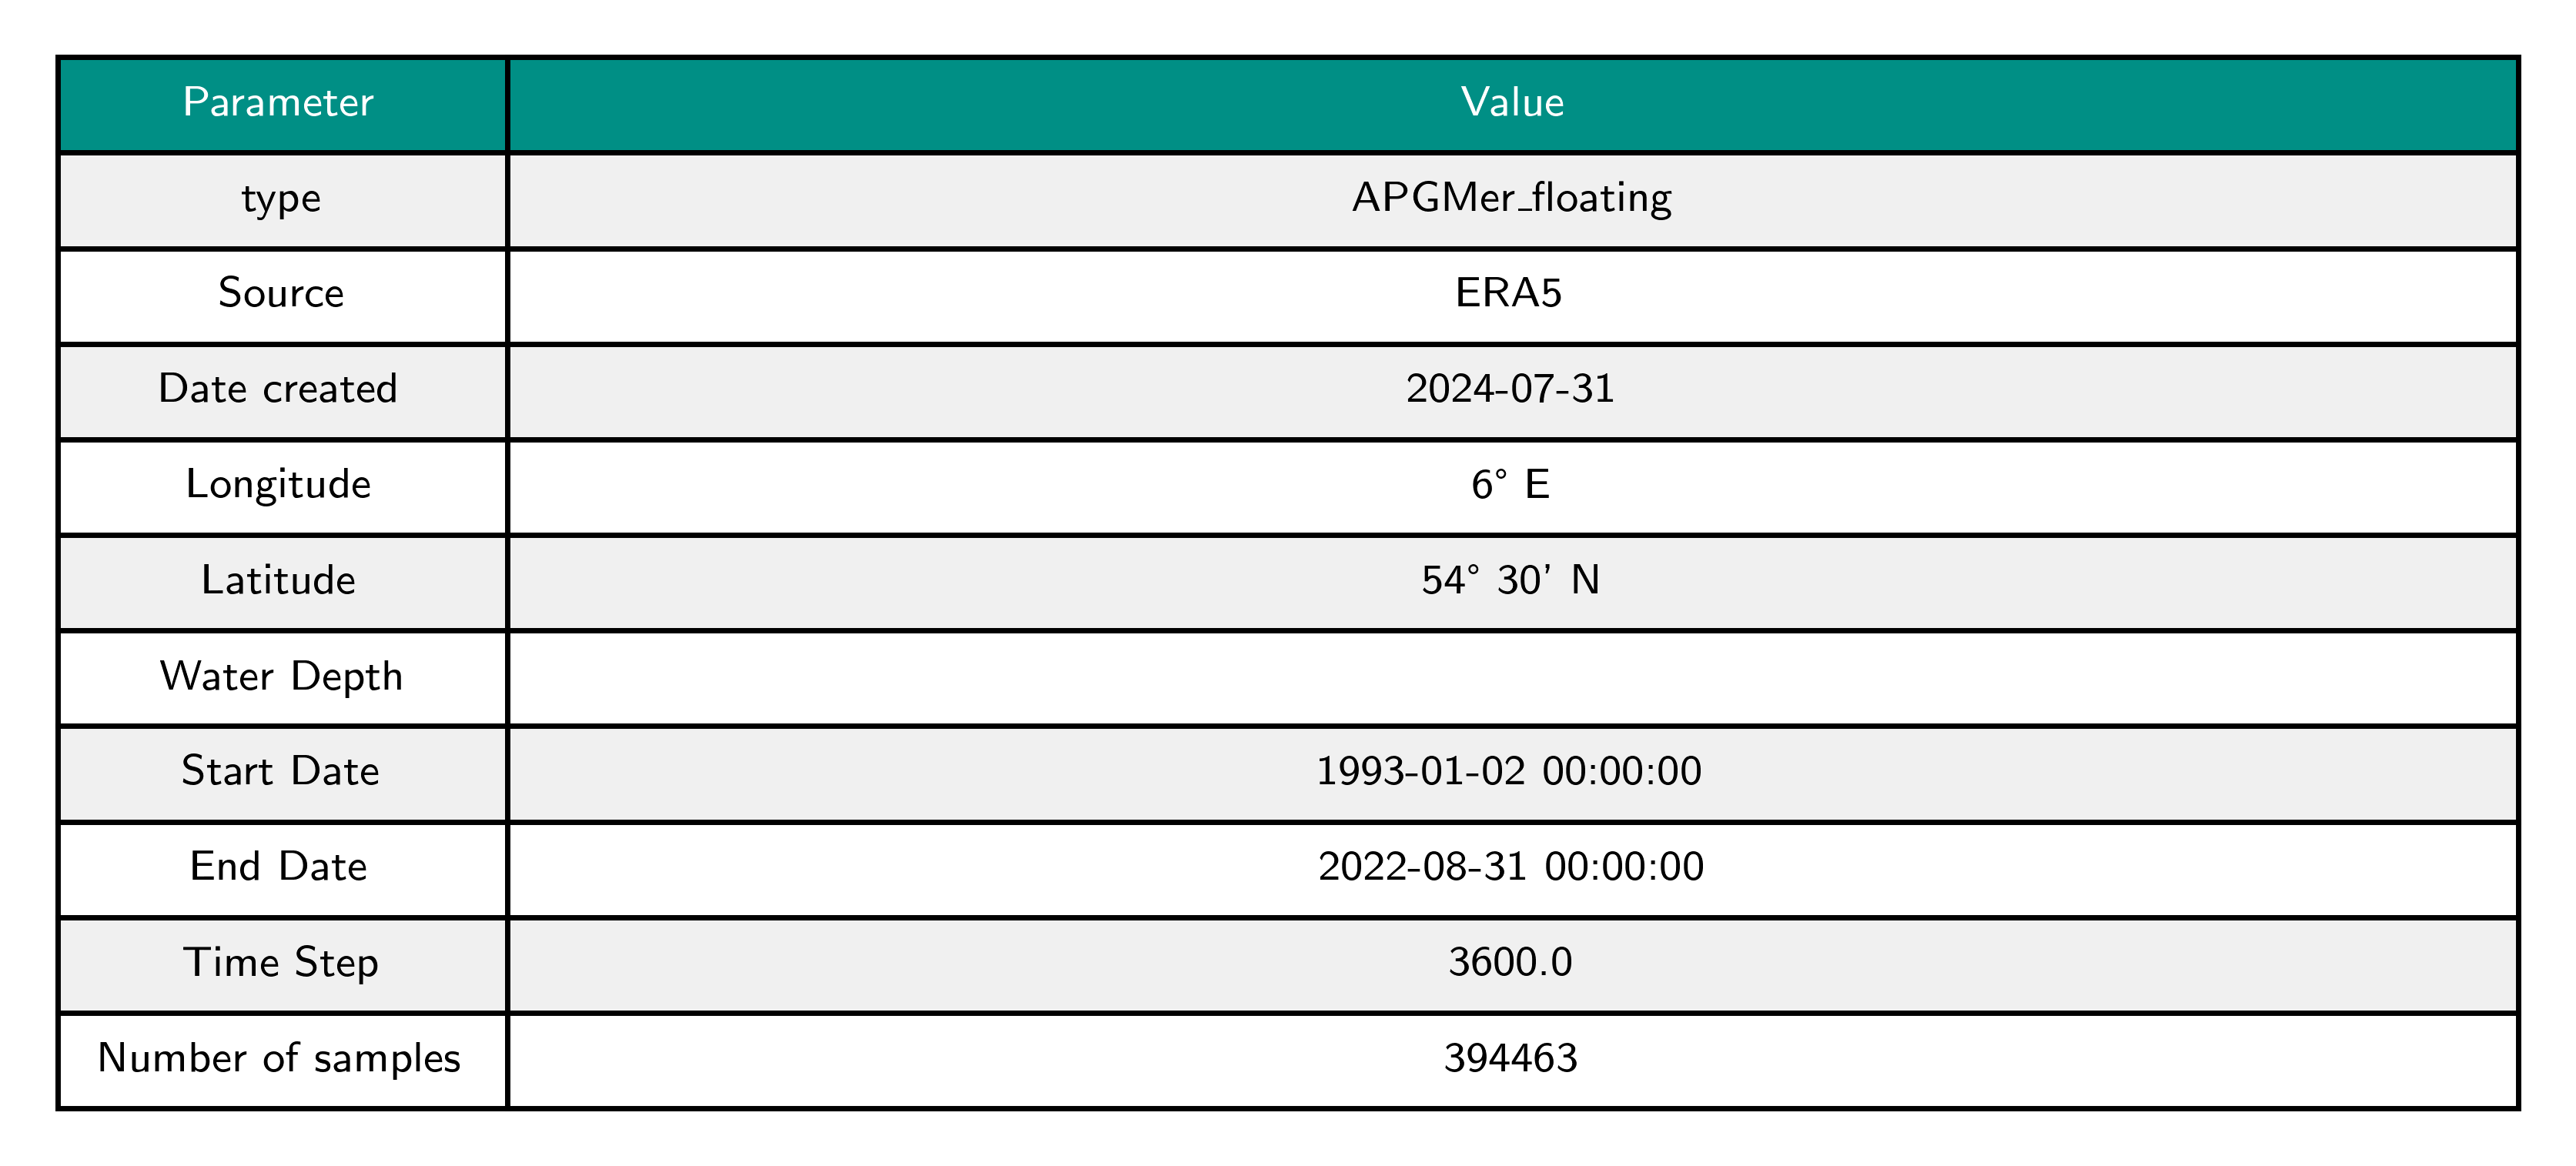
\includegraphics[width=1.0\textwidth ]{C:/Users/aaron.lange/Desktop/Projekte/Hindcast_Tool/HindTool/example_output/DataSorce_Waves_page_1.png} 
 \captionsetup{type=table} 
\caption{ DataSorce-Waves-page-1 } 
 \label{tab: DataSorce_Waves_page_1 } 
\end{figure}
\begin{figure}[H] 
 \centering 
 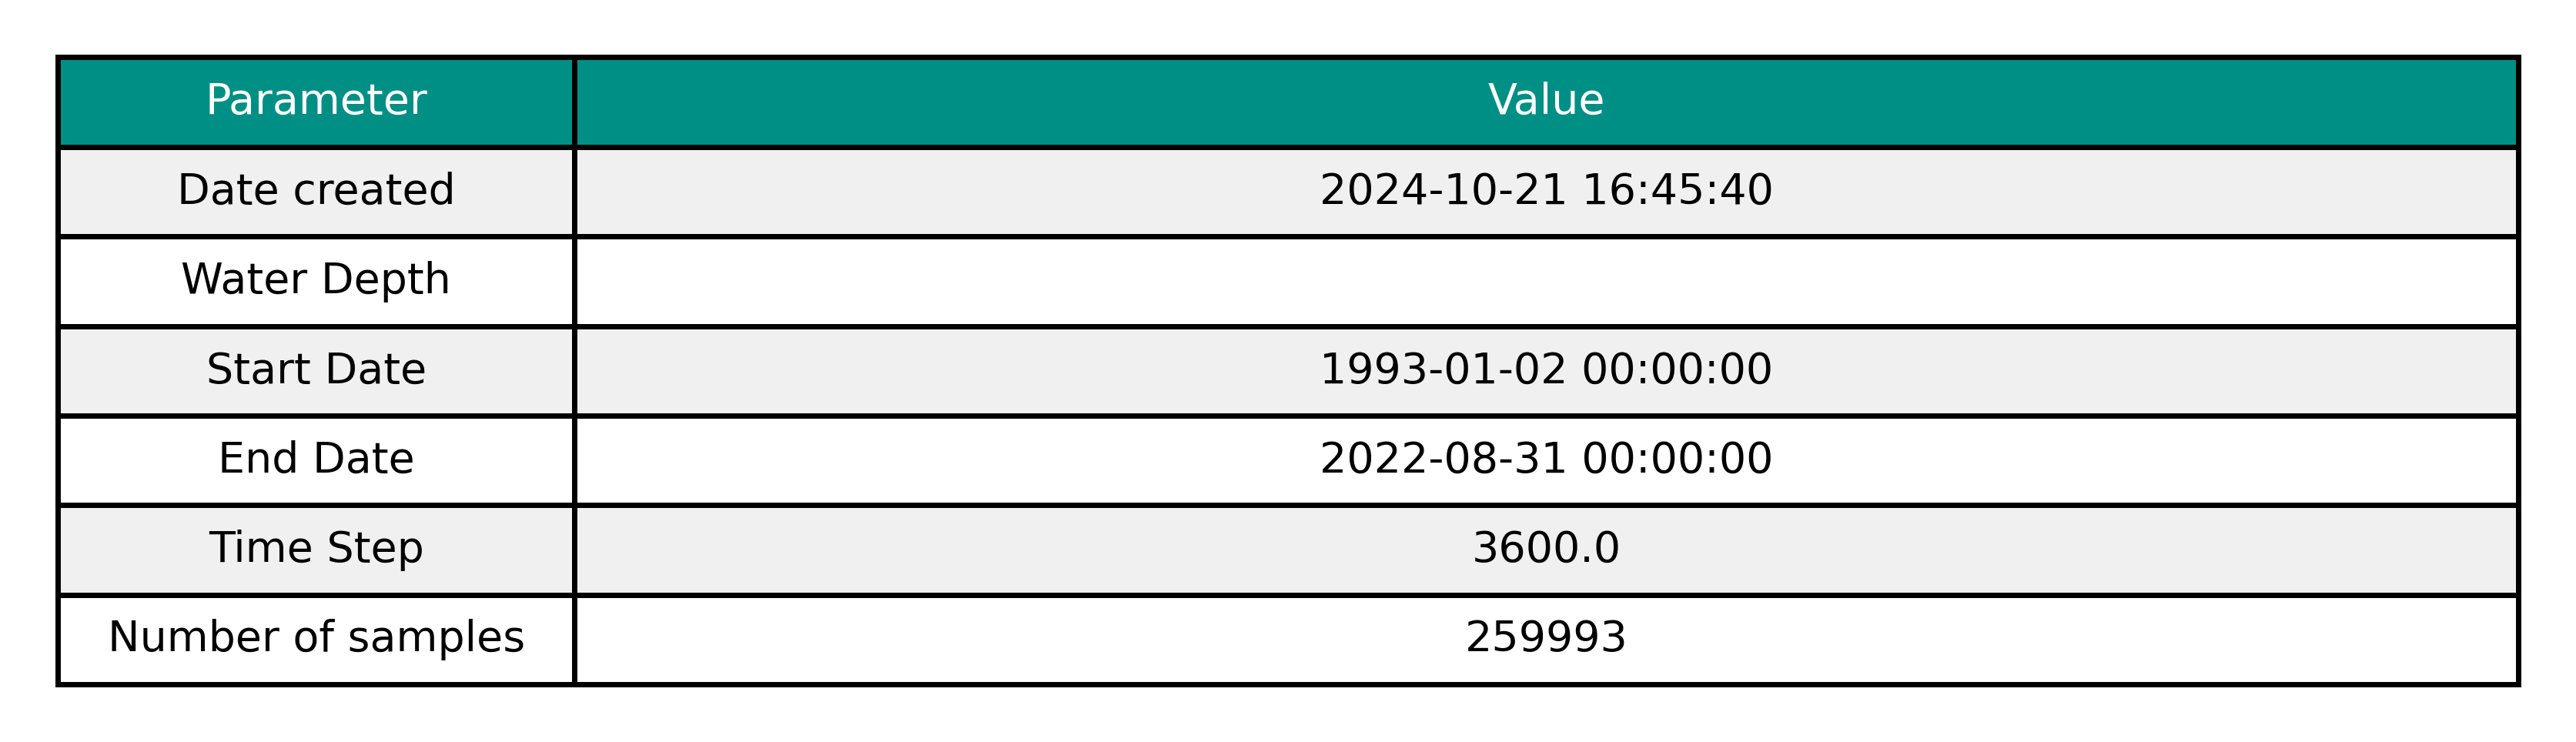
\includegraphics[width=1.0\textwidth ]{C:/Users/aaron.lange/Desktop/Projekte/Hindcast_Tool/HindTool/example_output/DataSorce_Winds_page_1.png} 
 \captionsetup{type=table} 
\caption{ DataSorce-Winds-page-1 } 
 \label{tab: DataSorce_Winds_page_1 } 
\end{figure}


\subsection{Data resampling} 
The timestep of 3600.0 s is chosen to be the timestep for all calculation. Deviating timesteps must be sampled down to be combined with the wave data. For this, the mean of all measurements corresponding to one timestep of wave data is used.
If the timeframes of the datasets are different, the timframe containing all data from the different databasis is choosen in the resampling step to keep all data. For the calculations, only the data present in all relevent databasis are loaded.  In the table below the sampling rates and the resulting numbers of samples as well as the timeframes of the original and the combined datasets are listed.

\begin{figure}[H] 
 \centering 
 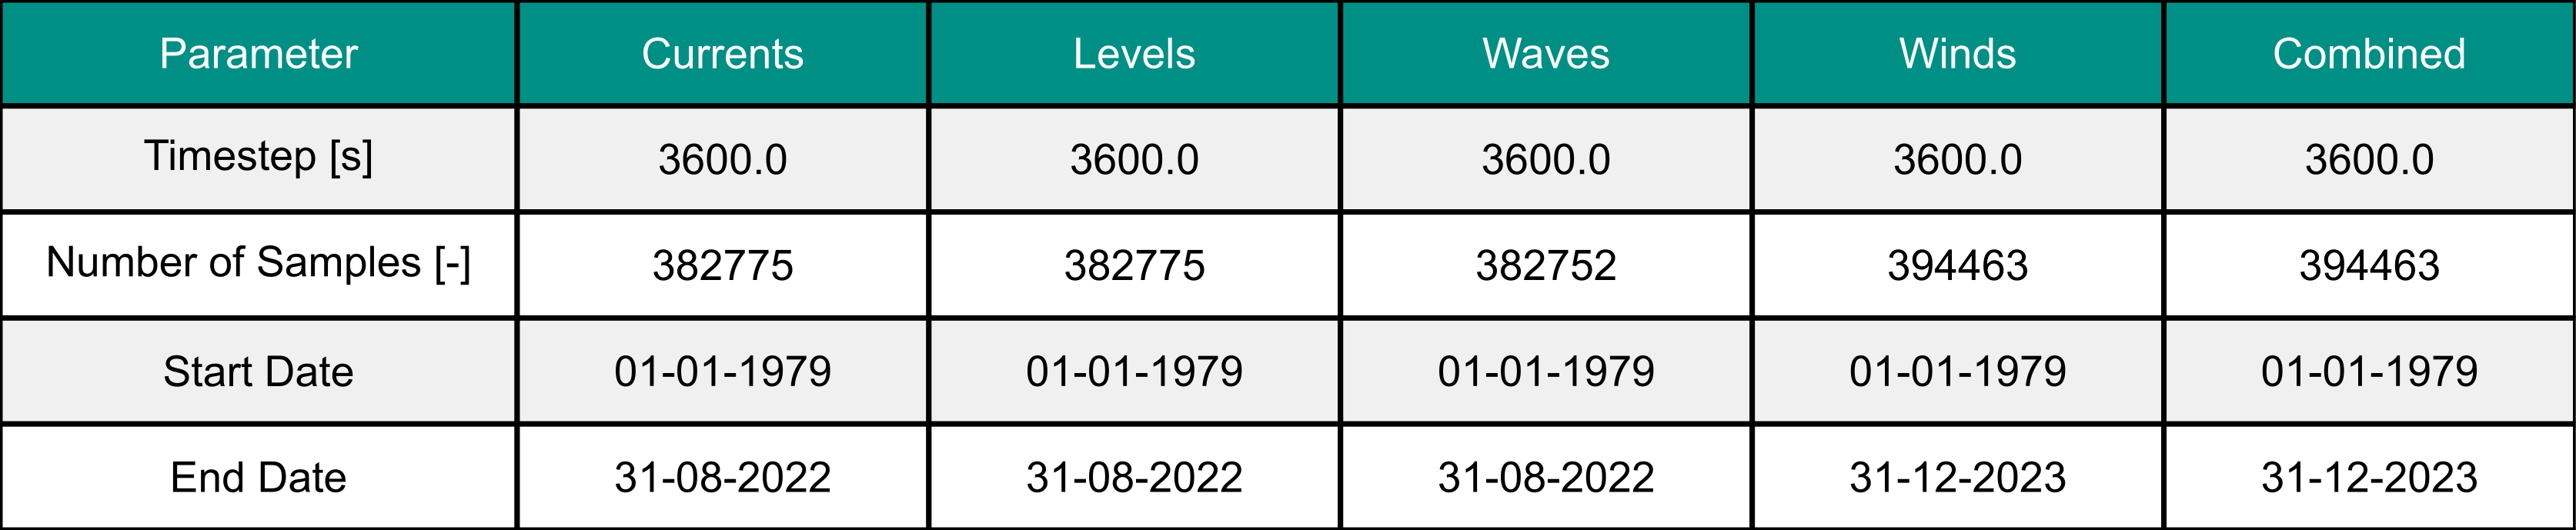
\includegraphics[width=1.0\textwidth ]{C:/Users/aaron.lange/Desktop/Projekte/Hindcast_Tool/HindTool/example_output/DataSorce_ResamplingTable_page_1.png} 
 \captionsetup{type=table} 
\caption{ DataSorce-ResamplingTable-page-1 } 
 \label{tab: DataSorce_ResamplingTable_page_1 } 
\end{figure}

\subsection{Filtering routines}
All rows containing 'nan' values in one of the relevant sensors are excluded from this specific calculation.  
Also, if the separated wind sea component is used extra filtering is necessary in case of the wind-wave missalignment. Because of the separation process of wind sea and swell, some components can be zero if there is no separable wind sea component. In this case, the wave period is zero as well and the wave direction can’t be determined anymore and is set to 0°, which also distorts the angle misalignment evaluations. For this reason, these sea states are excluded. 